\documentclass{article}
\usepackage[portuguese]{babel}
\usepackage[utf8]{inputenc}
\usepackage[T1]{fontenc}
\oddsidemargin -0.25in 
\evensidemargin -0.25in
\marginparwidth 40pt 
\marginparsep 10pt
\topmargin -0.25in 
\textheight 9.1in 
\textwidth 6.75in
\usepackage{fixltx2e}
\usepackage{setspace}	
\usepackage{amsmath}
\usepackage{enumerate}
\usepackage{booktabs}
\usepackage{graphicx}
\usepackage{multicol}
\usepackage{color}
\usepackage{capt-of}
\usepackage{mdwlist}
\usepackage{amssymb}
\providecommand{\abs}[1]{\lvert#1\rvert}
\usepackage{listings}
\usepackage{color}

\definecolor{mygreen}{rgb}{0,0.6,0}
\definecolor{mygray}{rgb}{0.5,0.5,0.5}
\definecolor{mymauve}{rgb}{0.58,0,0.82}

\lstset{ %
  backgroundcolor=\color{white},   % choose the background color; you must add \usepackage{color} or \usepackage{xcolor}
  basicstyle=\footnotesize,        % the size of the fonts that are used for the code
  breakatwhitespace=false,         % sets if automatic breaks should only happen at whitespace
  breaklines=true,                 % sets automatic line breaking
  captionpos=b,                    % sets the caption-position to bottom
  commentstyle=\color{mygreen},    % comment style
  deletekeywords={...},            % if you want to delete keywords from the given language
  escapeinside={\%*}{*)},          % if you want to add LaTeX within your code
  extendedchars=true,              % lets you use non-ASCII characters; for 8-bits encodings only, does not work with UTF-8
  frame=single,                    % adds a frame around the code
  keepspaces=true,                 % keeps spaces in text, useful for keeping indentation of code (possibly needs columns=flexible)
  keywordstyle=\color{blue},       % keyword style
  language=Octave,                 % the language of the code
  morekeywords={*,...},            % if you want to add more keywords to the set
  numbers=left,                    % where to put the line-numbers; possible values are (none, left, right)
  numbersep=5pt,                   % how far the line-numbers are from the code
  numberstyle=\tiny\color{mygray}, % the style that is used for the line-numbers
  rulecolor=\color{black},         % if not set, the frame-color may be changed on line-breaks within not-black text (e.g. comments (green here))
  showspaces=false,                % show spaces everywhere adding particular underscores; it overrides 'showstringspaces'
  showstringspaces=false,          % underline spaces within strings only
  showtabs=false,                  % show tabs within strings adding particular underscores
  stepnumber=2,                    % the step between two line-numbers. If it's 1, each line will be numbered
  stringstyle=\color{mymauve},     % string literal style
  tabsize=2,                       % sets default tabsize to 2 spaces
  title=\lstname                   % show the filename of files included with \lstinputlisting; also try caption instead of title
}

\begin{document}

\vskip -5mm
\onehalfspacing
\fbox{
  \begin{minipage}{0.4in} 
    
\includegraphics[scale=0.3]{images.png}\\~\\~\\
  \end{minipage}
  \begin{minipage}{6in}
    ~\\
    IST- MEFT - Física Computacional - 06/12/2014 ~~~~~~~~~~~~~~~~~~~~~~~~~~~~~~~~~~Pedro Pereira: 78889\\ 
    Prof. Fernando Barão~~~~~~~~~~~~~~~~~~~~~~~~~~~~~~~~~~~~~~~~~~~~~~~~~~~~~~~~~~~~~~~~~~~~~~~~~~ 
    João Alves: 79006 \\
    \textbf{Grupo B09}~~~~~~~~~~~~~~~~~~~~~~~~~~~~~~~~~~~~~~~~~~~~~~~~~~~~~~~~~~~~~~~~~~~~~~~~~~~~~~~ \\
    \begin{center} \textbf{2º Trabalho Física Computacional - Memória Descritiva}\linebreak \end{center}
  \end{minipage}
}

\medskip

\begin{abstract}
  Neste trabalho estudaram-se problemas físicos através de métodos numéricos. Foram tratados os cenários de molas acopladas verticalmente, a secção eficaz de interação de um neutrão com um núcleo em função da sua energia e de decaimentos radiativos. Para o problema das molas usaram-se métodos matriciais, para o da secção eficaz métodos de interpolação de dados e para o dos decaimentos métodos de Monte Carlo.
\end{abstract}





\begin{multicols}{2}
  \section{Molas Acopladas}
  \par  

  \subsection{Construtor}
  Neste problema, utilizou-se uma classe para resolver sistemas de equações possíveis e determinados, EqSolver. Esta possui três variáveis privadas, um array de arrays de doubles m (matriz dos coeficientes), um array de doubles b (vetor dos termos independentes), e um inteiro size, correspondente ao tamanho da matriz (quadrada). No construtor instanciaram-se estas de acordo com as variáveis dadas pelo utilizador.

  \subsection{M\'etodos}
  Neste problema usou-se a classe já desenvolvida em aula, EqSolver. Como tal, possui métodos não necessarios à resolução deste exercício, os quais não serão descritos aqui. Assim, fizeram-se dois métodos centrados  neste problema:\\

  \textbf{void LUdecomposition3(float *p,float *q,float *r,int n)}: Este metodo foi desenvolvido para proceder à fatorização LU de uma matriz. Assim, recebe três vetores de floats, correspondentes às três diagonais não-nulas da matriz, sendo $p$ a inferior e $q$ a principal, e um inteiro $n$, igual ao número de linhas (ou colunas, uma vez que a matriz tem de ser quadrada para possuir solução única). De seguida, procede-se à eliminação de gauss, guardando-se no vetor p os coeficientes usados nesta. É de notar que neste metodo os vetores $p$, $q$ e $r$ são alterados.\\

  \textbf{void LUsolve3(float *p,float *q,float *r,int n,double* z)}: Este método foi desenvolvido para resolver um sistema LU=z, no qual LU é a fatorização de uma matriz tridiagonal. Assim, recebe os três arrays de floats ($p$, $q$, $r$) correspondentes ao resultado da operação \textbf{LUdecomposition3}. Recebe ainda um inteiro $n$, igual ao numero de linhas de $LU$, e um array de doubles, $z$, correspondente ao vetor dos coeficientes independentes no sistema inicial $Ax = b$ a resolver.\\

  Começa-se por resolver $Ly = z$. Para se evitar retornar variáveis, declarou-se o metodo como void, operando diretamente sobre $z$. Para isso, aproveita-se o facto da primeira linha de $L$ ser um na primeira coluna e zero nas restantes, para afirmar que $y_0 = z_0$. De seguida, define-se recursivamente $y_k$, atraves da expressao $y_k = z_k - e_{k-1}y_{k-1}$. Visto se ter operado sobre $z$ diretamente, fez-se $z_k -= e_{k-1}y_{k-1}$, para $k = 1, ..., n-1$. Posto isto, resolveu-se $Ux = y$ (z neste caso), usando-se o facto de a ultima linha ser nula com excepção da última entrada. Assim, $z_{n-1} = q_{n-1}$. Desta forma, calcularam-se as restantes componentes de $x_n$ recursivamente, segundo a forma $z_k = \frac{z_k - r_kx_{k+1}}{q_k}$.

  \subsection{Sistema de Equações}

  Sendo que a equação de movimento para cada massa é dada por: 

  \begin{equation}
    m\ddot{x} = -K_n(x_n - x_{n-1}) + K_{n+1}(x_{n+1} - x_n) - m_ng
  \end{equation}

  E, numa situação de equilibrio, $\ddot{x} = 0$, obtém-se o seguinte sistema de equações na sua forma matricial, substituindo $K_n$ e $m_n$ pelos seus valores:

  \[
  \begin{bmatrix}
    20  & -10 &  0  &  0 &  0\\ 
    -10 & 20  & -10 &  0 &  0\\ 
    0   & -10 &  15 & -5 &  0\\ 
    0   &  0  & -5  & 10 & -5\\ 
    0   &  0  &  0  & -5 &  5
  \end{bmatrix}
  .
  \begin{bmatrix}
    x_{0}\\
    x_{1}\\
    x_{2}\\
    x_{3}\\
    x_{4} 
  \end{bmatrix}
  =
  \begin{bmatrix}
    100\\
    50 \\
    100\\
    50 \\
    100 
  \end{bmatrix}
  \]

  Cuja solução é dada por:

  \begin{equation}
    (x_0, x_1, x_2, x_3, x_4) = (40, 70, 95, 125, 145) mm
  \end{equation}

  \section{Interpolação de Dados}
  \par
  Como data members desta classe definiu-se N, o número de pontos, e os arrays de doubles x e y, tendo x as abcissas dos pontos da tabela e y as ordenadas.

  \subsection{Construtor}

  No construtor desta classe definiu-se um array de doubles temporário para onde se passaram os valores atribuídos na main. Posteriormente igualou-se este array temporário ao array correspondente dos data members. Procedeu-se desta forma para evitar memory leaks.

  \subsection{M\'etodos}
  \subsubsection{CubicSplineCurvatures}
  Ao realizar método CubicSplineCurvatures, verificou-se que a matriz a resolver era tridiagonal logo decidiu-se usar os métodos do EqSolver para o resolver. Verificou-se analiticamente que as diagonais não-principais(a e c) eram iguais, e que estas eram dadas por:  
  a[i]=(x[i+2]-x[i+1])/6; \\
  que a diagonal principal b, era dada por:
   b[i]=(x[i+2]-x[i])/3;\\
   e que o vetor indepedente,s, era dado por:
   s[i]=( (y[i+2]-y[i+1]) /(x[i+2]-x[i+1]) )-( (y[i+1]-y[i])/(x[i+1]-x[i])); \\
  
  O sistema a resolver foi, então:
  
\[
  \begin{bmatrix}
    50/3  & 25/6 &  0  &  0 &  0 & 0 & 0\\ 
    25/6 & 50/3  & 25/6 &  0 &  0& 0 & 0\\ 
    0   & 25/6 &  50/3 & 25/6 &  0& 0 & 0\\ 
    0   &  0  & 25/6  & 50/3 & 25/6& 0 & 0\\ 
    0   &  0  &  0  & 25/6 &  50/3& 25/6 & 0\\
    0 & 0  & 0 &  0 &  25/6& 50/3 & 25/6\\ 
    0   & 0 &  0 & 0 &  0& 25/6 & 50/3
  \end{bmatrix}
  .
  \begin{bmatrix}
    k_{1}\\
    k_{2}\\
    k_{3}\\
    k_{4}\\
    k_{5}\\
    k_{6}\\
    k_{7} 
  \end{bmatrix}
  =
  \begin{bmatrix}
    0.944\\
    0.38\\
    -2.768\\
    -0.088 \\
    0.952 \\
    0.262\\
    -0.04
  \end{bmatrix}
  \]

  Cuja solução é dada por:
$
  \begin{bmatrix}
    0.0417789\\
     0.0594444\\
      -0.188356\\
       0.029661\\
        0.0485922\\
        0.00445007\\
        -0.00351252
  \end{bmatrix}  
  $
  
  
  
  Tendo o vetor-solução criou-se outro a partir desse e com o primeiro e o último elemento a 0, visto o método garantir que a 1ª derivada é contínua e que as 2ªs derivadas se anulam nos extremos. 

  \subsubsection{CubicSplineSegment}
  Neste método definiu-se uma forma bastante simples de encontrar o intervalo a que pertence o ponto de teste. Após uma condição que filtra os pontos fora do domínio, temos um while que adiciona 1 ao iterador cada vez que se verifica que a abcissa do ponto de teste é maior que x[i]. Assim, assumindo um ponto de teste entre x[k] e x[k+1], i sairá do ciclo com o valor de k+1, ou seja, o indíce correspondente ao extremo superior. Como queremos o intervalo anterior, na atribuição dos parâmetros há que fazer uma correção, daí fazer-se:
  \begin{lstlisting}
    f->SetParameter(0,x[i-1]);
    f->SetParameter(1,x[i]);
    f->SetParameter(2,k[i-1]);
    f->SetParameter(3,k[i]);
    f->SetParameter(4,y[i-1]);
    f->SetParameter(5,y[i]);
  \end{lstlisting}

  \subsubsection{CubicSpline}
  Para este método usou-se o construtor de TF1 que recebe um functor. Verificou-se que pôr essa função auxiliar como membro da classe dava problemas, como tal, foi retirada e atribiu-se o primeiro valor do array de parametros ao número de pontos. Para escolher o segmento a usar usou-se o mesmo método de cima. Contudo, como o primeiro valor do array já esta atribuído, quando i=k temos par[k+1]=x[k], logo par[k] corresponde ao extremo inferior,  nao sendo assim necessário fazer a correção usada no método anterior, na atribuiçao dos parâmetros. \\
 \textbf{O Valor da Interpolaçao por Cubic Spline no ponto de Energia 57.3 é 59.2962 mbarn}. 

  \subsubsection{Polinómios}
  Achou-se útil do ponto de vista pedagógico tentar implementar todos os métodos dados em aula - Newton, Lagrange, Neville. Percebeu-se que havia duas formas possíveis de implemetar os métodos, através de functor ou de manipulação de strings. Para o de Newton e de Lagrange fez-se com manipulação de strings, isto é, criar ciclos que formam a expressão desejada para a função em formato string com posterior conversão para char* para o envio para o construtor de TF1. Para o de Neville usou-se o construtor de TF1 que recebe o functor. Neste, primeiro definem-se os polinómios de ordem zero, isto é, guardando num array os valores de y[i]. Depois cria-se um loop dentro de outro, sendo que o primeiro vai controlar a ordem do polinómio a ser retornado e o segundo, tendo em conta que é um método recursivo e vai usar os polinómios de ordens inferiores, os xk usados na aproximação polinomial de ordem inferior.
 Os 3 polinómios obtidos foram iguais, tal como seria de esperar, pois o polinómio interpolador é único.
   \\
 \textbf{O Valor da Interpolaçao por Polinómio no ponto de Energia 57.3 é 63.0119 mbarn}. 
  \subsubsection{CubicSplineDeriv}
  Neste método usou-se a mesma lógica de CubicSpline, sendo que desta vez se usou a expressão para a derivada, tal como apresentada na aula teórica.

  \subsubsection{Derivadas Numéricas}
  Nos métodos de derivadas numéricas após filtrar pontos fora do domínio seguem-se vários testes de extremos, sendo que, falhando todos a derivada a ser calculada será a central. Caso seja um ponto muito próximo de x[0] ou ele próprio, calcula-se a forward derivative, caso seja um ponto muito próximo de x[N] ou ele proprio, calcula-se a backward derivative. Não houve grande dificuldade na implementação destes métodos, visto que nos limitámo-nos a implementar as fórmulas dadas em aula teérica, após definir bem as condições para cada uma. Para calcular o valor das funções usou-se o método Eval do TF1.

  \subsubsection{Gráficos de Diferenças}
  Nestes métodos definiu-se um fator de escala, scaler, que iria determinar o número de pontos do gráfico. Caso fosse 1, o gráfico resumir-se-ia a algo com x[N-1] pontos, em que a diferença das abcissas entre eles seria de 1. Para uma visão mais nítida do gráfico definiu-se scaler como 10, sendo que a diferença entre abcissas sucessivas passa a ser x[N-1]/(x[N-1]*scaler), neste caso 0.1. Assim, preenche-se um array com o valor das diferenças, e outro com o valor do x correspondente, num ciclo que vai incrementando o x pelo valor previamente definido. Posteriormente enviam-se esses arrays para o construtor de TGraph, obtendo assim o gráfico desejado.

  \subsubsection{Problemas que Surgiram}
  O que levou mais tempo a assimilar foi a forma como o ROOT trabalha com o functor, tendo em conta que esse construtor do TF1 é um pouco criptíco. É algo estranho definir uma função com dois argumentos, chamando-a posteriormente sem os definir/atribuir duma forma explícita. Além disso, houve um problema pelo caminho relacionado com o cálculo dos k's. No fim de tudo, verificava-se que a diferença das derivadas do CubicSpline dava algo sem significado. Na determinação dos k's estava a ser cometido um erro derivado duma letra  trocada, mas que gerava um função de interpolação visualmente aceitável, escondendo a possibilidade dessa ser a fonte de erro. Foi daí que surgiu a criação da função que retorna a derivada do Cubic Spline em TF1*,algo sugerido pelo professor, onde se verificou que a derivada não era contínua, mostrando que havia um erro ou na definição do CubicSpline ou dos k's. Apresenta-se um gráfico desta, por se achar adequado. Só após se verificar todo o código (demasiadas vezes) e certificarmo-nos de que tudo era lógico é que se cogitou que o erro pudesse estar em funções à partida tomadas como certas. Apesar das dores de cabeça, esse erro foi bastante instrutivo e pedagógico para o futuro.\\  Já dizia Alberto Caeiro:
  "Ter Certeza é não estar vendo."

  \subsubsection{Resultado Final}
  \begin{center}
    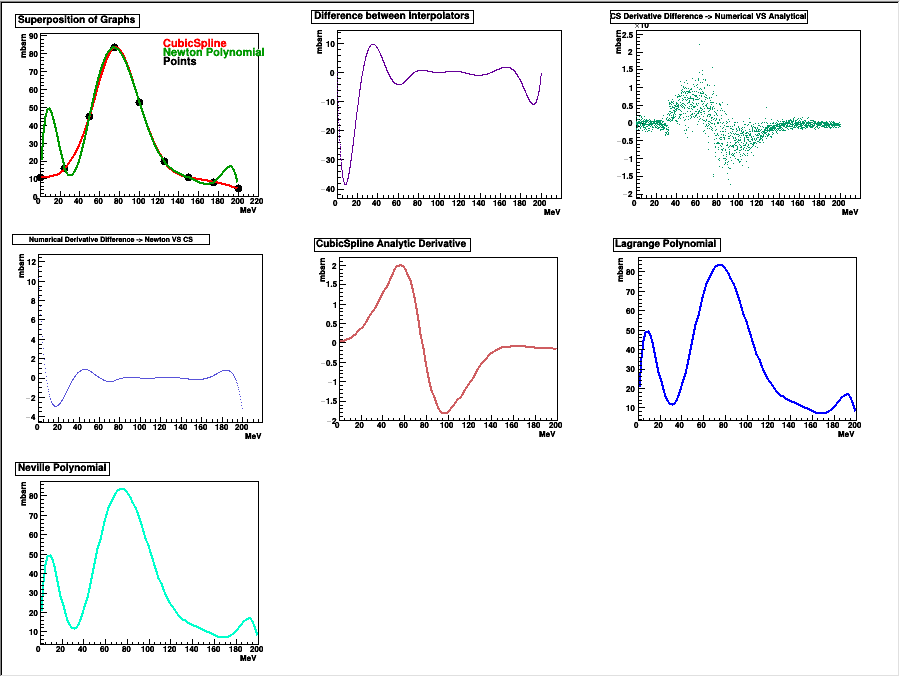
\includegraphics[scale=0.2]{resultados3.png}
    \captionof{figure}{Results}
  \end{center}

  \section{Decaimento Radioativo e Métodos de Monte Carlo}
  

  \subsection{Classes}

  \subsubsection{PhysProcess}

  A classe \textit{PhysProcess} é uma classe puramente virtual, que irá funcionar como classe mãe de todos os processos f+isicos. Guarda apenas o nome do processo.

  \subsubsection{BetaDecay e AlphaDecay}

Os objetos de ambas as classes sao instanciados de forma semelhante, quer através de um default constructor, quer de um construtor da forma \textit{BetaDecay (double a, double b)} ou \textit{AlphaDecay (double a, double b)}. Estas igualam as variáveis privadas T12 (tempo medio de vida, em segundos) e Q (energia cinética máxima do eletrão, em MeV), comuns a ambas as classes, a $a$ e $b$, respetivamente.\\

Para além de funções auxiliares, como a \textit{void SetT12(double)}, \textit{void SetQ(double)} e \textit{double GetT12()}, que permitem aceder às variáveis privadas da classe, esta possui duas outras com maior importância, a \textit{double Spectrum(double Te)}, que retorna o valor do espetro de um eletrão com energia cinética $Te$ (para o AlphaDecay esta função retorna sempre zero, visto nao ser conhecido o espetro desse decaimento) e a \textit{int DecayRate(int N, double t)}. Esta retorna o número de núcleos que decaíram de uma população com $N$ elementos no instante inicial, passados $t$ segundos.


  \subsubsection{Element}

  Esta classe armazena toda a informação disponível sobre um elemento. Possui dois construtores, um default, e outro, da forma \textit{Element (string,int,int,int)}, que permite inicializar as variáveis privadas desta classe de acordo com o pretendido pelo utilizador. Estas são: o nome do elemento - \textbf{string name}, número de nucleos - \textbf{int N}, número de massa - \textbf{int A} e número atómico - \textbf{int Z}. Esta possui ainda uma outra variável privada, \textbf{v}, que corresponde a um vetor de ponteiros para objetos PhysProcess. Assim, consegue-se armazenar no elemento qualquer processo físico que derive deste.\\

  Existem ainda duas funções auxiliares, \textit{void SetN(int)} e \textit{int GetN()}, que permitem tratar com a variável privada $N$, algo necessário no decorrer do exercício.

  \subsection{Sistema de equações diferenciais e solução analítica}

 \begin{equation}
 \begin{split}
  \begin{cases}
    dN_{Bi}=-\lambda_{Bi}N_{Bi}\\ 
    dN_{Po}+\lambda_{Po}N_{Po}=-dN_{Bi}
  \end{cases}
  =\\
  \begin{cases}
    N_{Bi}(t)=N_{0_{Bi}}e^{-\lambda_{Bi}t}\\ 
    N(t)_{Po}=\frac{-N_0\lambda_{Bi}}{\lambda_{Bi}-\lambda_{Po}}(e^{-\lambda_{Bi}t}-e^{-\lambda_{Po}t})
  \end{cases}
  \end{split}
  \end{equation}

  \subsection{Resolução do Exercicio}

  \subsubsection{Alinea 1}

  Neste caso, optou-se por utilizar intervalos de tempo diferentes para cada elemento, visto terem constantes de decaimento com ordem de grandeza diferente ($\lambda = \frac{log(2)}{T_{12}}$). Assim, procurou-se usar um tempo na mesma ordem de grandeza que $T_{12}$, de modo a observar o decaimento até perto da fase final, isto é, até ao momento em que todos os núcleos decaíram. Assim, usou-se $t = 20 dias$ para a população de Bismuto, e $t = 300 dias$, para a de Polónio. Note-se ainda que a probabilidade de decaimento de um átomo é dada por $dp = \lambda tdt$. Utilizando o metodo \textit{DecayRate}, fez-se sempre decair primeiro a população de Bismuto, sendo que o numero de núcleos que esta perdia a cada decaimento foi adicionado à população de Polónio, a qual iniciava seguidamente o seu processo de decaimento.

  \subsection{Alinea 2}

  Foram obtidos os seguintes gráficos para as populações de Polónio e Bismuto ao longo do tempo (apresentados apenas 2 como exemplo):

  \begin{center}
    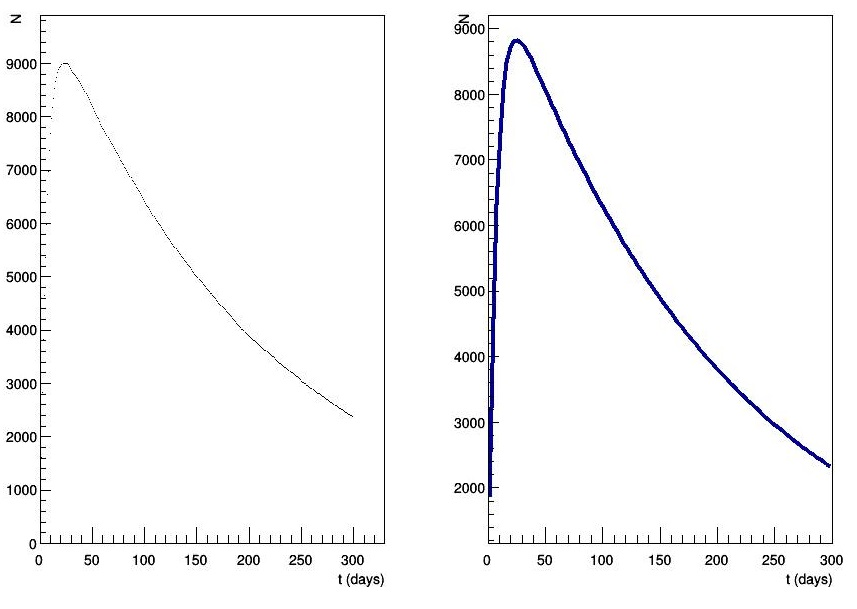
\includegraphics[scale=0.3]{DecayPo10000.jpg}
    \captionof{figure}{População do Polónio ao longo do tempo para $N_{Po}=0$ e $N_{Bi}=10000$, no intante inicial}
  \end{center}

\begin{center}
    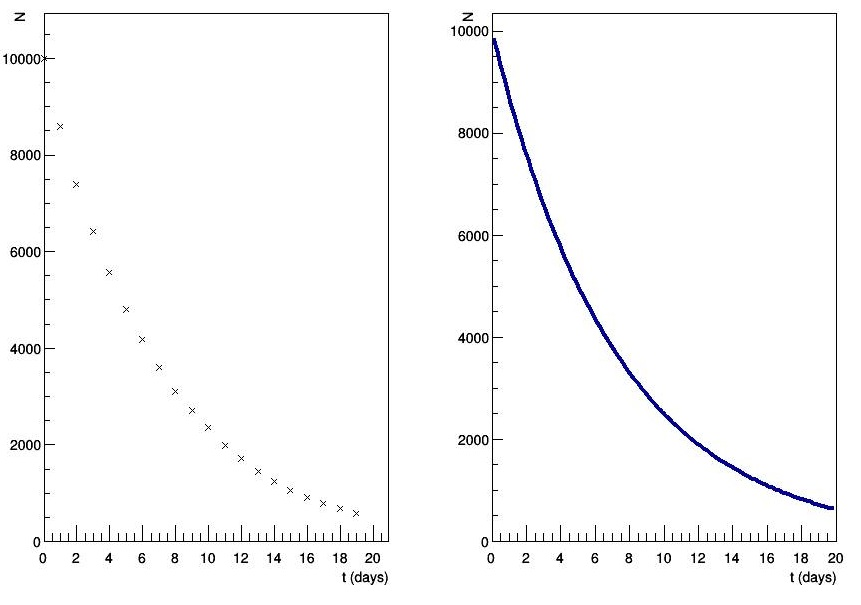
\includegraphics[scale=0.3]{DecayBi10000.jpg}
    \captionof{figure}{População do Bismuto ao longo do tempo para $N_{Po}=0$ e $N_{Bi}=10000$, no instante inicial}
  \end{center}
  
  Além disso, verificou-se que:\\
 \textbf{ Para N inicial 1000 tem-se 736 atomos de bismuto ao fim de 2 dias e 261 atomos de polónio.\\
Para N inicial 10000 tem-se 7482 atomos de bismuto ao fim de 2 dias e 2707 atomos de polónio.\\
Para N inicial 100000 tem-se 74203 atomos de bismuto ao fim de 2 dias e 27861 atomos de polónio.}


  \subsection{Alinea 3}

  Para se determinar o instante no qual é máxima a produção de particulas $\alpha$, limitou-se a verificar qual o instante para o qual decaíam mais elementos de Polonio, tendo sido $t = 19 dias$. Visto basear-se no método \textit{DecayRate}, da classe \textit{AlphaDecay}, a este valor está associado uma grandeza aleatória, pelo que irá variar de cada vez que se corra o programa.
  
  \subsection{Alinea 4}
  Apresentam-se seguidamente os gráficos gerados:
\begin{center}
    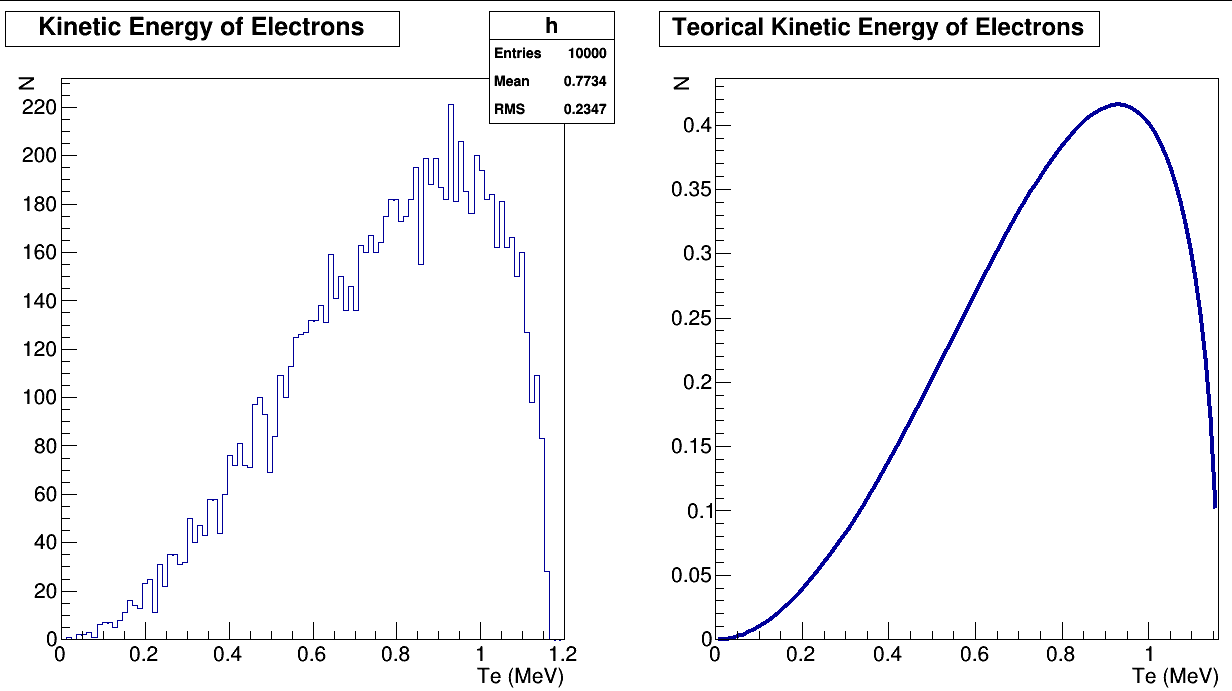
\includegraphics[scale=0.2]{eletro.png}
    \captionof{figure}{Gráfico das Energias dum eletrão geradas aleatoriamente à esquerda, à direita o teórico.}
  \end{center}
  \subsection{Alinea 5}

  Começou-se por notar que, visto a função $N(T_e)$ apenas estar definida de 0 a 1.1612, expandiu-se a função fora deste como sendo igual a zero, pelo que o integral passou a ser calculado apenas entre estes valores.

  No integral de Monte Carlo, utilizou-se a seguinte distribuição de probabilidade:

  \[
  f(x) =
  \begin{cases}
    0.05 \leftarrow 0 <= x < 0.3\\ 
    \frac{sin(3.4995x + \phi)}{I} \leftarrow 0.3<= x <= 1.1612\\
  \end{cases}\]

  Em que, $\phi = asin(0.05)-3.4995*0.3$ e $I = \frac{1-0.05*.3}{cos(0.3*3.4995+phi)-cos(1.1612*3.4995+phi)}$.\\

  Assim, conseguiu-se aumentar a eficácia do integral. Para conseguir uma precisão abaixo de 0.001, foi necessário utilizar 100000 aleatórios.\\

  No caso do integral de Simpson, houve dificuldades na obtenção de um majorante para o erro. Isto prendeu-se com o facto de qualquer derivada da função tender para $-\inf$ quando $x$ tendia para 1,1612. Assim, definiram-se duas funções em escada, $M(x)$ e $m(x)$, constantes para cada intervalo de largura $\frac{1.1612}{n}$, sendo n o numero de intervalos. M(x) teria como valor em cada intervalo o máximo da função, e m(x) o mínimo, nesse intervalo. Uma vez que o polinómio utilizado no integral de simpson está contido entre ambos, tal como a função, o erro do integral de simpson pode ser majorado pelo integral de $(M-m)(x)$. Para garantir que este erro é menor que 0.001, foi necessário usar como largura de cada intervalo $\frac{1.1612}{2300}$. É de notar que o valor exato do erro para este valor será bastante menor, visto a majoração ser bastante grosseira.\\
\textbf{Os valores obtidos, foram, então:\\
Simpson: 0.602026 com erro de 0.00096592\\
MC: 0.602407 com erro de 0.00039894}\\


  \subsection{Alinea 6}

  Para calcular a energia média do eletrão detetável, integrou-se a seguinte expressão:

\begin{equation}
  N(T_e)\varepsilon (T_e)T_e
\end{equation}
\textbf{e o resultado foi:
0.401866 MeV}


  \begin{thebibliography}{9}


  \bibitem{Procedimento}
    \textit{Stroustrup, Bjarne. The C++ Programming Language. Reading, MA: Addison-Wesley, 2013.}
  \bibitem{Procedimento}
    \textit{Barão, Fernando. Slides das Aulas Teóricas. 2014.}

  \end{thebibliography}
\end{multicols}
\end{document}
